\documentclass[12pt, a4paper]{article}
\usepackage{graphicx}
\usepackage{mathtools}
\usepackage{xcolor}
\usepackage{amsmath}
\usepackage{caption}
\usepackage[italian]{babel}
\usepackage{eso-pic}
\usepackage{setspace}
\usepackage{multirow}
\usepackage{array}
\usepackage{geometry}
\usepackage{longtable}
\graphicspath{ {./immagini/} }
\linespread{1.1}
\binoppenalty=10000 %impedisce di separare a capo formule matematiche nel testo
\relpenalty=10000
\geometry{
 total={170mm,257mm},
 left=20mm,
 top=15mm,
 bottom=28mm
 }
\title{\textbf{\scalebox{1.4}{\text{Misura di g tramite il pendolo}}}}
\date{}

\begin{document}
\maketitle
\AddToShipoutPictureBG*{%
  \AtPageUpperLeft{%
    \hspace{\paperwidth}%
    \raisebox{-\baselineskip}{%
      \makebox[0pt][r]{\textbf{Gruppo 10}: Mussini Simone, Musi Francesco, Ruscillo Fabio        }
}}}%


\section{Richiami teorici}
Il pendolo semplice è un sistema costituito da un filo inestensibile di lunghezza $L$ di massa trascurabile a cui è appesa una massa $m$, che all'occorrenza può essere spostata dalla posizione verticale di equilibrio e dare origine ad un moto oscillatorio. 

Trascurando l'attrito con l'aria, sulla massa agisce soltanto la forza peso. 
L'equazione del moto si ottiene egualiando la compnente normale della forza rispetto al filo, alla formula generica per la forza centripeta di un moto circolare con raggio = $L$.
Risulta essere un moto armonico soltanto per le piccole oscillazioni, cioè quando si può approssimare $sin(\theta) = \theta$, dove $\theta$ è l'angolo che il filo forma con la verticale. 

\begin{equation}
        F_t = -mg sin(\theta)\hat{t} = mL\ddot{\theta}   \quad \xrightarrow{} \quad   \frac{d^2\theta}{dt^2} = -\omega^2\theta 
\end{equation}

Dove $\omega = \sqrt{\frac{g}{L}}$ è la pulsazione, che dipende non dalla massa $m$, ma soltanto dalla lunghezza del filo e accelerazione di gravità. 

Il periodo di una oscillazione risulta: $T = \frac{2\pi}{\omega} = 2\pi\sqrt{\frac{L}{g}}$.



\section{Obbiettivi}
Gli obbiettivi di questo esperimento sono: 
verificare l'indipendenza del periodo $T$, tenendo $L$ costante, dall'ampiezza delle oscillazioni e dalla massa;
verificare la relazione quadratica tra $L$ e $T$; 
verificare il valore $g$ tramite na linearizzazione (quadratica) della legge del periodo.




\section{Strumenti}
    \begin{itemize}
        \item Piedistallo 
        \item filo inestensibile
        \item Masse calibrate
        \item Cronometro 
        \item Goniometro 
    \end{itemize}


    
\section{Procedimento di misura}
Il setup dell'esperimento è costituito da un piedistallo a cui è collegato un filo inestensibie regolabile in lunghezza tramite una vite. Nell'estremità superiore è presente un goniometro, solidale con il piedistallo, che permette di sapere l'angolo delle oscillazioni. All'estremità inferiore del filo è collegata una spilla che permette di variare la massa appesa. \\
Disponiamo di 5 masse che pesano: 66.3g, 37.2g, 22.2g, 16.8g, 12.5g.

Sui dati presi con il cronometro, consideriamo l'errore umano nella misura dei tempi, ossia un decimo di secondo, maggiore dell'errore strumentale. 
Nella misura degli angoli con il goniometro, tenimao l'errore strumentale. 

Abbiamo notato che la lunghezza del filo, aumenta all'aumentare della massa. Tuttavia la discrepanza tra allungamento massimo e minimo è minore della somma dei rispettivi errori ($\pm0.2cm$ su ogni misura), quindi possiamo approssimarlo a filo inestensibile.

Le masse le assumiamo note essendo l'ordine di grandezza dell'errore relativo trascurabile.

Per aumentare la precisione delle misure, è opportuno misurare 10 periodi alla volta.
Infatti, visto che un periodo è nell'ordine di 1 secondo, misurando un oscillazione alla volta, con l'errore umano si avrebbe un errore relativo dell'ordine del 10\%, troppo alto.
Invece essendo $10T$ nell'ordine di 10 secondi, l'errore relativo scende all'1\% circa.

È importante anche avere $L > 1m$, in modo che le oscillazioni non siano troppo brevi, sempre per tenere basso l'errore relativo.



\section{Misura di T}
\subsection{Stima dell'ordine di grandezza dell'errore di T}
Il cronometro con sui si sono registrati i tempi, ha una sensibilità al centesimo di secondo, ed inoltre i tempi di reazione umani sono dell'ordine del decimo di secondo. L'ordine di grandezza del periodo del pendolo per piccole oscillazioni, considerando un filo di lunghezza $L\approx (1,000\pm 0.001)\ m$, e usando $g_{tab}=(9.80665\pm0.00001) \ m/s^2$, è
\begin{equation*}
    T= 2\pi\ \sqrt{\frac{L}{g_{tab}}}\approx 2.00\ s
\end{equation*}
Per cui $T\approx(2.0\pm 0.1)s$ (considerando l'errore umano) dal quale si calcola un errore relativo sul periodo pari a
 \begin{equation*}
     \frac{\Delta T}{T}=5.0\%
 \end{equation*}
Poichè il moto è periodico, si può sfruttare il fatto che misurando $10T\approx(20.0\pm 0.1)\ s$, l'errore relativo sul periodo diventa $\displaystyle \frac{\Delta T}{T} = 0.5\% $
\newpage



\subsection{Distribuzione Gaussiana}
\label{gaussiana}
Si verifica che le misure di $10T$ seguano effettivamente una distribuzione Gaussiana, effettuando $N=30$ misure con la stessa massa $M=0.0222 \ kg$.
Fissati $L=(1.097\pm 0.002)\ m$ , $g_{tab}=(9.80665\pm 0.00001)\ m/s^2$ e $\Phi_{max}=8^o$ si riportano i dati nella seguente tabella: 


\begin{table}[!htb]
    \begin{minipage}[t]{.5\linewidth}
    \centering
        \begin{tabular}{|c|c|}
            \hline
            $10T$ $(s)$&$N$\\
            \hline
            $20.67\pm 0.01$ & $1$\\
            $20.72\pm 0.01$ & $1$\\
            $20.76\pm 0.01$ & $1$\\
            $20.87\pm 0.01$ & $1$\\
            $20.93\pm 0.01$ & $1$\\
            $21.00\pm 0.01$ & $2$\\
            $21.07\pm 0.01$ & $1$\\
            $21.09\pm 0.01$ & $2$\\
            $21.13\pm 0.01$ & $2$\\
            $21.14\pm 0.01$ & $1$\\
            $21.16\pm 0.01$ & $2$\\
            \hline
        \end{tabular}
    \end{minipage}
    \begin{minipage}[t]{.5\linewidth}
    \centering
        \begin{tabular}{|c|c|}
            \hline
            
            $21.20\pm 0.01$ & $1$\\
            $21.25\pm 0.01$ & $2$\\
            $21.26\pm 0.01$ & $3$\\
            $21.27\pm 0.01$ & $1$\\
            $21.33\pm 0.01$ & $2$\\
            $21.42\pm 0.01$ & $1$\\
            $21.43\pm 0.01$ & $1$\\
            $21.52\pm 0.01$ & $2$\\
            $21.59\pm 0.01$ & $1$\\
            $21.78\pm 0.01$ & $1$\\
            &\\
            \hline
            \hline
            TOT & 30\\
            \hline
        \end{tabular}
        \label{TAB:1}
        %\caption{aa}
    \end{minipage} 
\end{table}


\begin{center}
   \href{Tabella 1} : \textit{\footnotesize{Nella prima colonna sono riportati i valori registrati di 10T, nella seconda la frequenza delle singole misure.}}
\end{center}
\addvspace{2cm}


Tramite l'uso della calcolatrice si sono ottenuti i seguenti valori
\smallskip

\begin{itemize}
    \item\phantom{a} Valore medio:\phantom{aaaaaaaaa.aa}
          $\overline{x}=\overline{10T}=21.18633$
    \item\phantom{a} Deviazione standard:\phantom{aaaaa}
        $\sigma_x=0.2537$
    \item\phantom{a} Numero di vincoli:\phantom{aaaaaaaa}$\upsilon=1$
    \item\phantom{a} Test del chi quadro:\phantom{aaaaaaa}$\chi^2=0.19577$ 
\end{itemize}
\bigskip

Quindi possiamo caloclare l'errore sul valor medio e l'errore relativo:
\begin{equation*}
    \Delta (\overline{10T})=\frac{\sigma_x}{\sqrt{N}}=0.046\approx 0.05s \quad ; \quad \frac{\Delta(\overline{10T})}{\overline{10T}} = 0.00236 \approx 0.24\%
\end{equation*}

Il valore percentuale dell'errore relativo ha lo stesso ordine di grandezza della stima fatta nel paragrafo precedente (0.5\%), pertanto lo possiamo ritenere corretto.



\newpage
\begin{figure}[h!]
    \centering
    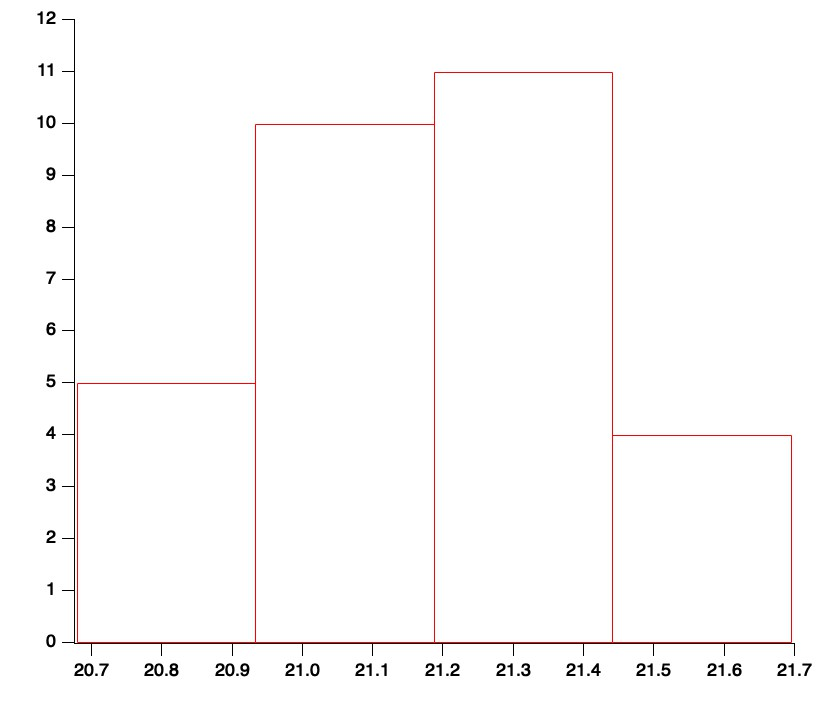
\includegraphics[width=130mm]{Immagini/Histogram Pendolo.jpg}
    \caption{\textit{{\footnotesize{L'Istogramma presenta 4 classi, ciascuna con la relativa frequenza (asse $y$) }}}}
    \label{Grafico parabolico}
\end{figure}

\bigskip
Questo è l'istogramma che si ottiene suddividendo i dati in 4 classi, ognuna con ampiezza di una deviazione standard.
La \textit{confidenza} ottenuta, consultando la relativa tabella, è compresa tra il 25\% ed il 50\%, quindi i valori di $10T$ misurati sono compatibili con un campione Gaussiano.
\bigskip







\section{Misura di M}
Tramite una bilancia elettronica con sensibilità al decigrammo, sono state pesate le masse campione:

\begin{table}[!htb]
    \centering
        \begin{tabular}{|c|c|}
            \hline
            $N^o$ &Massa M $(kg)$\\
            \hline
            $1$ & $0.0125\pm0.0001$\\
            $2$ & $0.0168\pm0.0001$\\
            $3$ & $0.0222\pm0.0001$\\
            $4$ & $0.0372\pm0.0001$\\
            $5$ & $0.0663\pm0.0001$\\
            \hline
        \end{tabular}
        \label{Tab masse}
        \caption*{Tabella 2: \textit{\footnotesize In Tabella sono riportate le masse campione, in ordine crescente.}}
        \end{table}

    Si considerano le masse come note, quindi con ordine di grandezza dell'errore relativo $<0.1\%$. Per questa ragione, si assumono le masse aventi incertezza nulla.



    
\section{Misura di L}
\label{Misura di L}
Si è poi passati al calcolo della lunghezza del filo al variare della massa appesa. Le misure registrate, tramite un metro a nastro con sensibilità al millimetro, sono le seguenti:

\begin{table}[!htb]
    \centering
        \begin{tabular}{|c|c|c|}
            \hline
            $N^o$ &Massa M $(kg)$&Lunghezza L $(m)$\\
            \hline
            $0$ & $0.0000$         &$1.094\pm0.002$\\
            $1$ & $0.0125\pm0.0001$&$1.095\pm0.002$\\
            $2$ & $0.0168\pm0.0001$&$1.096\pm0.002$\\
            $3$ & $0.0222\pm0.0001$&$1.097\pm0.002$\\
            $4$ & $0.0372\pm0.0001$&$1.099\pm0.002$\\
            $5$ & $0.0663\pm0.0001$&$1.103\pm0.002$\\
           
            \hline
        \end{tabular}
        \label{Tab Lunghezze}
        \caption*{\centering Tabella 3: \textit{\footnotesize Sono riportate le masse campione e le diverse lunghezze del filo misurate. L'errore di 2mm è dovuto alla distanza da tenere tra il metro ed il filo per non muovere quest'ultimo.}}
        \end{table}


Come si può osservare dalla Tabella 3, la lunghezza del filo a riposo è $L_0=(1.094\pm0.002)\ m$. Si noti come tutte le lunghezze siano confrontabili, tranne quella corrispondente alla $N^o\ 5$, che vale $L_5=(1.103\pm0.002)\ m$. Questo può essere dovuto al fatto che il filo utilizzato fosse diventato più cedevole a casua degli utlizzi precedenti. Tuttavia la discrepanza tra l'allungamento massimo e quello minimo è minore dell'1\% della lunghezza media, quindi la trascuruiamo.\\

La lunghezza media del filo $\overline{L}$ è:

\begin{equation*}
    \overline{L}=\frac{\sum_{i=1}^{5}L_i}{5}=1.096\ m \quad , \quad
    \Delta \overline{L}=0.020\ m
\end{equation*}
\bigskip

Quindi $\overline{L}=(1.096\pm0.020)\ m$







\section{Indipendenza di T da $\Phi_{max}$}
\label{Indip T da angolo}

Per mostrare in quale intervallo angolare vale l'indipendenza di T dall'ampiezza massima, sono state effettuate 6 misure di dieci periodi, mantenendo la stessa massa $M=(0.0663\pm0.0002)\ kg$ durante tutte le misurazioni, e variando l'angolo, misurato tramite un goniometro posto all'estremità dell'asta rigida che sorregge il pendolo. 
\bigskip

Le misure sono state fatte per angoli di $\Phi_{max1}=(5^o\pm1^o)$, $\Phi_{max2}=(10^o\pm1^o)$, $\Phi_{max3}=(15^o\pm1^o)$, $\Phi_{max4}=(20^o\pm1^o)$, $\Phi_{max5}=(25^o\pm1^o)$, $\Phi_{max6}=(30^o\pm1^o)$.\\

Esiste una formula che permette di calcolare il periodo anche per angoli per cui non vale l'approssimazione $sin(\Phi) = \Phi$, che sfrutta uno svilupo in serie, come segue:

\begin{equation}\label{sviluppo periodo}
    T=T' \left(1+\frac{1}{4}\ \sin^2{\left(\frac{\Phi_{max}}{2}\right)}\right)
\end{equation}

dove il termine $T'$ è il periodo calcolato per angoli piccoli, ed è dato da:
\begin{equation}
T'=2\pi\ \sqrt{\frac{{L}}{g}}
\end{equation}
\bigskip




\begin{table}[ht] 
\centering
\begin{tabular}{|c|c|c|c|c|c|c|} 
 \hline
    &$\Phi_{max1}\ (^o)$ & $\Phi_{max2}\ (^o)$ & $\Phi_{max3}\ (^o)$ & $\Phi_{max4}\  (^o)$ & $\Phi_{max5}\ (^o)$ & $\Phi_{max6}\ (^o)$  \\
    &$(5\pm1)$ & $(10\pm1)$ & $(15\pm1)$ & $(20\pm1)$ & $(25\pm1)$ & $(30\pm1)$  \\
\hline
    $10T$& $21.31\pm 0.05 $&$21.30\pm0.05$&$21.25\pm0.05$&$21.19\pm0.05$ &$21.16\pm0.05$&$21.60\pm 0.05$\\
\hline
    $T$& $2,13\pm 0.01 $&$2.13\pm0.01$&$2.12\pm0.01$&$2.12\pm0.01$ &$2.12\pm0.01$&$2.16\pm 0.01$\\
\hline
\end{tabular}\\



\caption*{\centering Tabella 4: \small{\textit{Sono riportati i dati delle misure al variare dell'angolo, graficati successivamente.}}}
    \label{tab T indip Angolo}
\end{table}





\begin{figure}[h!]
\centering
\includegraphics[width=160mm]{Immagini/Grafico Angolo Periodo.jpg}
\caption{\textit{{\footnotesize{La retta rossa indica la compatibilità sicuramente dei primi 3 dati, e anche dei successivi 2. }}}}
\label{confrontoTT'}
\end{figure}

Come si può vedere in Figura \ref{confrontoTT'}, fino ad una angolo $\Phi_{max5}=15^o$ il periodo misurato risulta pienamente compatibile, quindi indipendente dall'angolo. All'aumentare dell'ampiezza $T$ si discosta sempre più dai primi 3 dati, pur restando compatibile nella terza e quarta misura.\\

Nel calcolo dell'equazione del moto di un pendolo, otteniamo l'espressione per angoli piccoli approssimando $sin(\Phi) = \Phi$. 
Se $\Phi = 10^o$ essi coincidono fino alla terza cifra decimale, mentre se $\Phi = 15^o$ fino alla seconda. 
I valori del periodo misurati hanno una precisione dell'ordine di $10^{-2}$ quindi è corretto che le prime 3 misure siano così simili. 






\newpage
\section{Indipendenza di T da M}
\label{Indip T da M}
Si effettuano 5 misurazioni di $10T$, ciascuna con una massa diversa. Si è scelto di far partire l'oscillazione da un angolo fisso pari a $\Phi_{max}=8^o$, così da non avere una dipendenza di $T$ dall'angolo, come mostrato nella Sezione \ref{Indip T da angolo}, e con una lunghezza del filo costante pari a $\overline{L}=(1.096\pm0.020)\ m$, risultato ottenuto nella Sezione \ref{Misura di L}.\\

I risultati sono riportati in tabella:


DATI DA INSERIRE IN TABELLA!!!!!!!!!!!!!! NON SONO QUELLI GIUSTI

\begin{table}[ht] 
\begin{tabular}{|c|c|c|c|c|c|} 
\hline
    &$M1\ (kg)$ & $M2\ (kg)$ & $M3\ (kg)$ & $M4\ (kg)$ & $M5\ (kg)$   \\
    &\small$(0.0125\pm0.0001)$ & \small$(0.0168\pm0.0001)$ & \small$(0.0222\pm0.0001)$ & \small$(0.0372\pm0.0001)$ & \small$(0.0663\pm0.0001)$ \\
\hline
    $10T$& $21.31\pm 0.05 $&$21.30\pm0.05$&$21.25\pm0.05$&$21.19\pm0.05$ &$21.16\pm0.05$\\
\hline
    $T$& $2,13\pm 0.01 $&$2.13\pm0.01$&$2.12\pm0.01$&$2.12\pm0.01$ &$2.12\pm0.01$\\
\hline
\end{tabular}\\


\caption*{\centering Tabella 5\small{\textit{ } }}
    \label{tab T indip Angolo}
\end{table}

    \begin{figure}[h!]
\centering
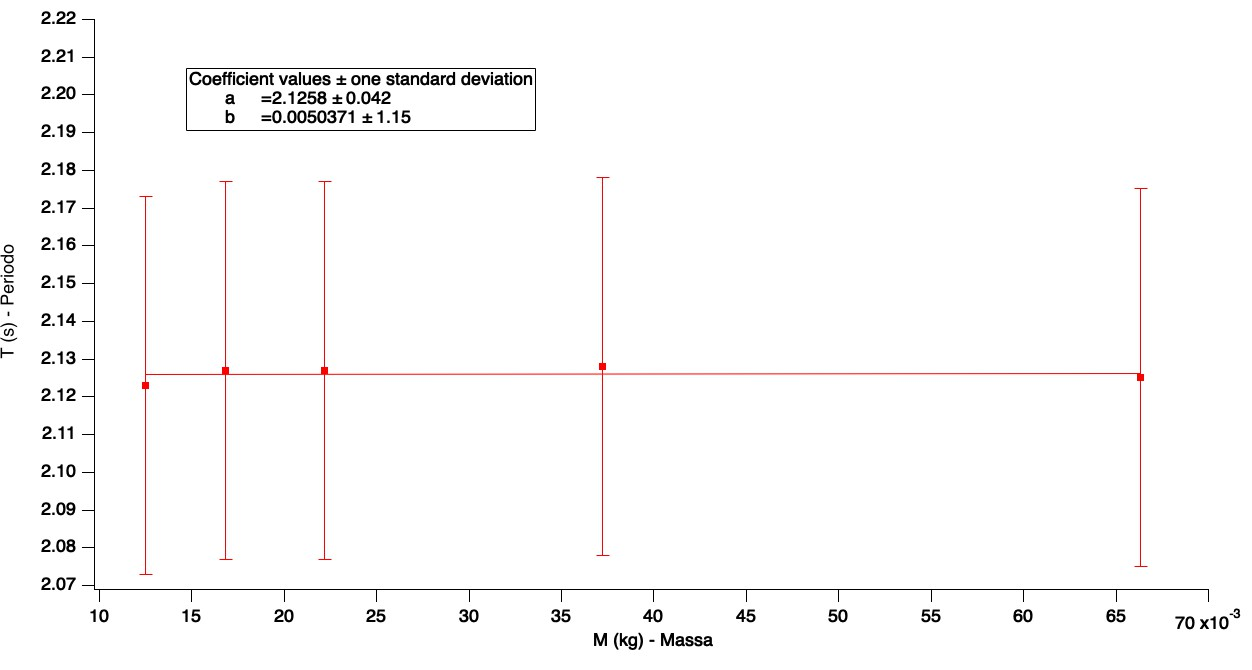
\includegraphics[width=170mm]{Immagini/IndipTdaM.jpg}
\caption{\textit{{\footnotesize{descrizione  }}}}
\label{IndipendenzaTM}
\end{figure}


Come si può notare dal Grafico \ref{IndipendenzaTM}, $T$ rimane pressochè costante al variare di $M$ e come conseguenza la retta ottenuta dal \textit{Quick Fit} è orizzontale con pendenza $b=(0.0\pm1.2)$.

Si è quindi verificata l'indipendenza di $T$ da $M$. 







\newpage
\section{Dipendenza di T ed L}
\label{Dip TL}
Si sono eseguite ulteriori misure di $10T$, però modificando la lunghezza del filo dopo ogni misura. Quest'ultima è stat presa misurado la distanza tra il supporto e l'inizio della massa. Successivamente si è sommata la lunghezza di metà pesetto, ottenendo così la distaza tra punto di vincolo e centro di massa: $\displaystyle L=L_{mis}+\frac{h}{2}$.
Si riportano i valori misurati ed il grafico da essi formato:


\begin{table}[h!]
    \centering
    \begin{tabular}{|c|c|c|}
    \hline
        $ L \pm \Delta L (m) $ & $ 10T \pm \Delta10T (s)$ & $ T \pm \Delta T(s)$  \\ 
    \hline 
    $1.025 \pm 0.003$ & $20.29 \pm 0.05$ & $2.03 \pm 0.01$\\ 
    $1.075 \pm 0.003$ & $20.71 \pm 0.05$ & $2.07 \pm 0.01$\\ 
    $1.125 \pm 0.003$ & $21.30 \pm 0.05$ & $2.13 \pm 0.01$\\ 
    $1.175 \pm 0.003$ & $21.57 \pm 0.05$ & $2.16 \pm 0.01$\\ 
    $1.225\pm 0.003$ & $22.01 \pm 0.05$ & $2.20 \pm 0.01$\\ 
    $1.275 \pm 0.003$ & $22.61 \pm 0.05$ & $2.26 \pm 0.01$\\ 
    $1.325 \pm 0.003$ & $23.19 \pm 0.05$ & $2.32 \pm 0.01$\\ 
    $1.375 \pm 0.003$ & $23.54 \pm 0.05$ & $2.35 \pm 0.01$\\ 
    $1.425 \pm 0.003$ & $23.98 \pm 0.05$ & $2.40 \pm 0.01$\\ 
    $1.475 \pm 0.003$ & $24.21 \pm 0.05$ & $2.42 \pm 0.01$\\
    $1.525 \pm 0.003$ & $24.68 \pm 0.05$ & $2.47 \pm 0.01$\\
    \hline 
    \end{tabular}
    \caption*{\centering Tabella 6:\small{\textit{Periodo misurato al variare di L}}}
    \label{tab:my_label}
\end{table}



\begin{figure}[h!]
    \centering
    \includegraphics[width=170mm]{Immagini/Grafico LT lineare.jpg}
    \caption{\textit{{\footnotesize{Grafico di T in funzione di L.}}}}
    \label{IndipendenzaTM}
\end{figure}


A prima vista si potrebbe pensare che tra $T$ ed $L$ ci sia una relazione lineare, ma per esserne sicuri si effettua una \textit{Regressione Lineare}.






\subsection{Regressione lineare}
Successivamente si è fatta una regressione lineare, partendo da $T= \frac{2\pi}{\sqrt{g_{tab}}}\sqrt{L}$. Quello che ci si aspetta di trovare è che il periodo abbia una relazione di potenza pari ad $\frac{1}{2}$ con la lunghezza del filo. Seguono i dati ed il grafico.

Posti $ln(A) = a$, $B = b \quad \xrightarrow{} \quad T = A L^B$;
passando ai logaritmi si ottiene:
\begin{equation*}
    \ln{(T)}=a +b\ \ln{(L)} \quad , \quad     \Delta\ln{(T)}=\frac{\Delta T}{T}\ 
\end{equation*}



\begin{table}[h!]
    \centering
    \begin{tabular}{|c|c|}
    \hline
    $ln(L) \pm \Delta ln(L) $ & $ln(T) \pm \Delta ln(T) $  \\  
    \hline
    $ 0.025 \pm 0.003$ & $ 0.708\pm 0.005$ \\
    $ 0.072 \pm 0.003$ & $ 0.728\pm 0.005$ \\
    $ 0.118 \pm 0.003$ & $ 0.756\pm 0.005$ \\
    $ 0.161 \pm 0.003$ & $ 0.769\pm 0.005$ \\
    $ 0.203 \pm 0.002$ & $ 0.789\pm 0.005$ \\
    $ 0.243 \pm 0.002$ & $ 0.816\pm 0.004$ \\
    $ 0.281 \pm 0.002$ & $ 0.841\pm 0.004$ \\
    $ 0.319 \pm 0.002$ & $ 0.856\pm 0.004$ \\
    $ 0.354 \pm 0.002$ & $ 0.877\pm 0.004$ \\
    $ 0.389 \pm 0.002$ & $ 0.884\pm 0.004$ \\
    $ 0.422 \pm 0.002$ & $ 0.904\pm 0.004$ \\
    \hline
    \end{tabular}
    \caption*{\centering Tabella 7:\small{\textit{Valori calcolati per la regressione lineare}}}
    \label{tab:my_label}
\end{table}


\smallskip
\begin{figure}[h!]
    \centering
    \includegraphics[width=160mm]{Immagini/Grafico logaritmico.jpg}
    \caption{\textit{{\footnotesize{Valori logarirmici graficati}}}}
    \label{IndipendenzaTM}
\end{figure}

Il valore di $b$ è compatibile col valore $\frac{1}{2}$, esponente della lunghezza del filo nella formula usata in partenza.  Si è così dimostrato che vi è una relazione di potenza tra $T$ e $L$.







\newpage
\section{Misura di g}
Si è in fine proceduto al calcolo di $g$. Per prima cosa, poichè nella formula del periodo, $g$ è sotto radice, eleviamo al quadrato sia a destra che a sinistra dell'uguale e otteniamo:
\begin{equation*}
    T^2=4\pi^2\ \frac{L}{g}
\end{equation*} 
Isolando da un lato $\frac{L}{g}$ e si può definire una nuova variabile $Y$ con relativo errore:
\begin{equation*}
  Y=\frac{L}{g} \quad , \quad  Y=\frac{T^2}{4\pi^2} \quad , \quad \Delta Y=\frac{d}{dT}\left(\frac{T^2}{4\pi^2}\right)\Delta T=\frac{2T}{4\pi^2}\ \Delta T
\end{equation*}
Si utilizzano le misure della lunghezza $L$ e del periodo $T$ ottenuti nella Sezione \ref{Dip TL}, e si colcola $Y$ e $\Delta Y$. I dati sono tabulati e graficati successivamente.

 \begin{table}[!h]
    \centering
    \begin{tabular}{|c|c|c|}
    \hline
    $ L \pm \Delta L (m)$ & $ T \pm \Delta T (s) $  & $ Y \pm \Delta Y (s^2) $  \\ 
    \hline 
    $1.025 \pm 0.003$ & $2.03 \pm 0.01$ & $ 0.104 \pm 0.001$ \\ 
    $1.075 \pm 0.003$ & $2.07 \pm 0.01$ & $ 0.109 \pm 0.001$ \\ 
    $1.125 \pm 0.003$ & $2.13 \pm 0.01$ & $ 0.115 \pm 0.001$ \\ 
    $1.175 \pm 0.003$ & $2.16 \pm 0.01$ & $ 0.118 \pm 0.001$ \\ 
    $1.225 \pm 0.003$ & $2.20 \pm 0.01$ & $ 0.123 \pm 0.001$ \\ 
    $1.275 \pm 0.003$ & $2.26 \pm 0.01$ & $ 0.130 \pm 0.001$ \\ 
    $1.325 \pm 0.003$ & $2.32 \pm 0.01$ & $ 0.136 \pm 0.001$ \\ 
    $1.375 \pm 0.003$ & $2.35 \pm 0.01$ & $ 0.140 \pm 0.001$ \\ 
    $1.425 \pm 0.003$ & $2.40 \pm 0.01$ & $ 0.146 \pm 0.001$ \\
    $1.475 \pm 0.003$ & $2.42 \pm 0.01$ & $ 0.148 \pm 0.001$ \\
    $1.525 \pm 0.003$ & $2.47 \pm 0.01$ & $ 0.155 \pm 0.001$ \\
    \hline
    \end{tabular}
    \caption*{\centering Tabella 8:\small{\textit{Valori da graficare, nuova variabile definita}}}
    \label{tab:my_label}
\end{table}
 

\begin{figure}[h!]
    \centering
    \includegraphics[width=160mm]{Immagini/Grafico Misura di g.jpg}
    \caption{\textit{{\footnotesize{grafico con nuova vairabile Y}}}}
    \label{IndipendenzaTM}
\end{figure}


\newpage
Si è infine passati al calcolo di $g$ con rispettivo errore:
\begin{equation*}
    g=\frac{1}{b}=9.8039\frac{m}{s^2} \quad , \quad     \Delta \frac{1}{b^2}\Delta b=0.208\approx 0.2\ \frac{m}{s^2}
\end{equation*}
Quindi il valore dell'accelerazione di gravità risultate è $g=(9.8\pm0.2)$ $\frac{m}{s^2}$.

\addvspace{1cm}
Questo valore risulta compatibile con il valore tabulato $g_{tab}=(9.80665\pm 0.00001)\ m/s^2$ in quanto la discrepanza tra i 2 valori è minore della somma degli errori:

\begin{equation*}
    |g-g_{tab}|=6.65\cdot 10^{-3} \ \frac{m}{s^2}  \quad , \quad  |\Delta g-\Delta g_{tab}|=0.2\ \frac{m}{s^2}\\
\end{equation*}
\begin{equation*}
    \xrightarrow{} |g-g_{tab}|<< |\Delta g-\Delta g_{tab}|
\end{equation*}








\newpage
\section{Conclusioni}
Si è iniziato l'esperimento stimando l'errore di grandezza relativo sulla misura del periodo (5\%) e quello su $10T$ (0.5\%). In questo modo lo abbiamo confrontato con l'errore ottrenuto dall'analisi del campione gaussiano effettuato con le 30 misure del punto \ref{gaussiana}.
Nonostante i calcoli abbiano rilevato un errore minore di quello atteso (curca la metà), gli ordini di grandezza coincidono, pertanto si può accettare questa misura di T.\\

Successivamente sono state pesate le masse in dotazione e l'allungamento del filo con ciascuna di esse. 
Abbiamo riscontrato un allungamento al variare della massa maggiore di quello che ci saremmo aspettati, probabilmente dovuto ad un filo usurato, le cui fibre sono diventate più cedevoli. 

Visto che senza la supposizione di un filo instensibile l'esperimento non avrebbe senso, e visto che la variazione di lunghezza è comunque molto piccola rispetto alla lunghezza media del filo, decidiamo di trascuare questo effetto. È stato assunto come valore corretto della lunghezza la media tra le 5 minsure con il rispettivo errore medio. Si veda il paragrafo \ref{Misura di L} per calcoli più precisi.\\

Nelle misure per stabilire l'indipendenza del periodo dall'ampiezza massima è stato riscontrato, come i calcoli suggerivano, che fino a 15° non si sono verificate modifiche rilevanti nel periodo. 

Tuttavia ci saremmo aspettati che il periodo aumentasse all'auumentare dell'angolo, perchè il secondo termine dell'equazione (\ref{sviluppo periodo}) è $\frac{1}{4}sin^2(\frac{\Phi_{max}}{2})$, una quantità sicuramente positiva. Ciò è accaduto solo nell'ultima misura, mentre per 20° e 25° il periodo è diminuito. 
Attribuiamo queste incongruenze ad errori nelle misure, che sono state prese soltanto una volta, senza fare una media tra più ripetizioni della stessa situazione.\\


Nella verifica della non-relazione tra periodo e massa, invece, le misure effettuate sono molto ben confrontabili tra loro. Le righe verticali che rappresentano l'incertezza del periodo sono così alte perchè quest'ultima è di 2 ordini di grandezza superiore rispetto a quella della massa.\\

La misura della dipendenza tra T ed L ha richiesto una regressione lineare sui dati misurati, in quanto va verificato che $T \propto \sqrt{L}$.
Nonostante il grafico potesse ingannare, il programma di calolo ha verificato che sussista una relazione tra i nostri dati compatibile a quella attesa. 
Nell'immagine la linea che congiunge i dati appare una retta, ma in realtà è un arco di parabola con raggio di curvatura molto esteso.\\


COSA ABBIAMO FATTO?????????
Il risultato ottenuto è compatibile con il dato tabulato come mostrano i calcoli fatti.


\end{document}
